%!TEX root = ../dissertation.tex
\chapter{Definitions}
Here we present some of definitions of concepts and terms that are used throughout this work.

\subsection{Rules}
Rules are IF-THEN statements consisting of a boolean antecedent and a classification label.
We are working in the realm of binary classification, so the label is either a 0 or a 1.
The boolean antecedents are generated from the rule mining mechanism and can be a conjunction of boolean clauses.
These antecedents are satisfied by some data points and not for others.
We say a rule \textit{classifies} a given data point when the antecedent is satisfied for that data point.
As we combine these rules into rule lists, only the first rule that classifies any given data point can make a prediction for that data point.
Thus, we say a rule \textit{captures} a given data point if it is the first rule in a rule list to classify that data point.

\subsection{Rule Lists}
%Let us define a training dataset of size N as $\{x_n, y_n\}_{n=1}^N$ where each $x_n \in \{0, 1\}^J$ are binary features and each $y_n \in \{0, 1\}$ are binary labels.
%Each rule $x_n$ therefore classifies some of the data points (those indices where $x_{n, j} = 1$).
%Define a rulelist $\mathbf{r} = (r_1, r_2, ... , r_k, r_0)$ where each $r_i \in \{x_n\}_{n=1}^N, \forall i > 0$.
%$r_0$ is defined as the default rule, which makes a prediction on all data points that are not captured in rules $1 ... k$. 
A rule list is an ordered collection of rules.
As defined above, rules have inherent accuracies based on what data they classify and how they predict the label, but that they are judged based on what data they capture.
However, they can perform better or worse than their inherent accuracy depending on what rules come before them in a given rule list.
Thus, any model building technique is focused on finding a rule list that maximizes predictive accuracy.
A rule list also has a \textit{default rule}, placed at the end of all of the pre-mined rules, that classifies all data points and predicts the majority label.
We refer to the set of rules that compose a rule list, not including the default rule, as a \textit{prefix}.
A rule list makes prediction for all points because any point not captured by the prefix is therefore captured by the default rule.

\begin{figure}[t!]
%\vspace{-3mm}
\begin{algorithmic}
\normalsize
\State \bif $(age=23-25) \wedge (priors=2-3)$ \bthen $yes$
\State \belif $(age=18-20)$ \bthen $yes$
\State \belif $(sex=male) \wedge (age=21-22)$ \bthen $yes$
\State \belif $(priors>3)$ \bthen $yes$
\State \belse $no$
\end{algorithmic}
%\vspace{-3mm}
\caption{An example rule list that predicts two-year recidivism for the ProPublica dataset, found by CORELS.}
\label{fig:rule-list}
\end{figure}

\subsection{Objective}
Rule lists have a loss function based on the number of points that are misclassified by the rules in the rule list.
We define our objective function to be the sum of that loss and a regularization term.
We use a regularization term, which is a constant times the length of the rule list, to prevent our rule lists from growing too long and therefore losing their interpretability.
This objective function is what we are going to optimize over, and it is inversely correlated to the accuracy of the rule list. 

\subsection{Bounds}
We use the discrete-optimization technique of branch-and-bound to solve this combinatorially difficult problem.
This requires tight bounds that allow us to prune as much of the search space as possible.
These bounds are formalized and proved in Angelino et al. \cite{AngelinoLaAlSeRu17} and are listed in Appendix A.
For clarity's sake we present summaries of the important bounds here.

\subsubsection{Lower Bound}
We use the term \textit{lower bound} to mean the best possible outcome for the objective function for a given prefix.
We do this by calculating the error of the prefix and assuming that any points uncaptured by the prefix will be predicted correctly.
Because any future extensions of the prefix can never do better than this lower bound, we will be able to use it to prune our exploration.

\subsubsection{Objective Bound}
The first, and most important bound, is the objective bound.
This is the main bound for the branch-and-bound that says that we do not need to purse a rule list if it has a lower bound on its objective that is worse than the best objective we have already seen.
This allows us to prune large parts of the search space by not pursuing rule lists that could never be better than something we've already seen.

\begin{figure}
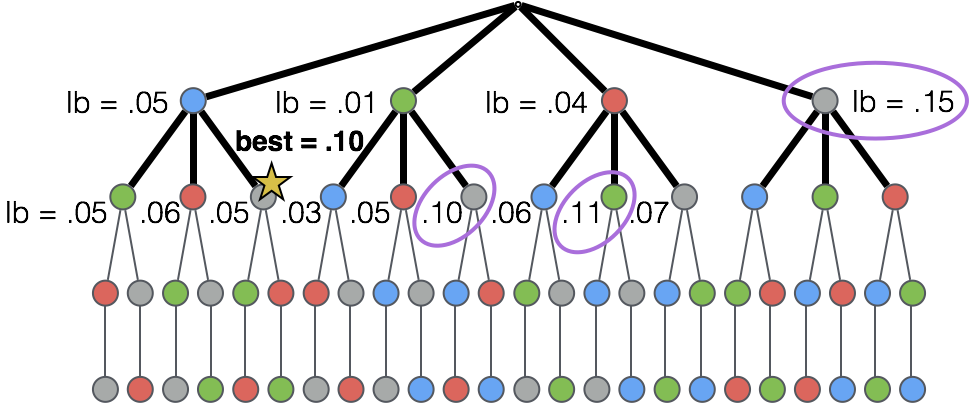
\includegraphics[width=0.5\textwidth]{figs/ela_branch-and-bound-tree.png}
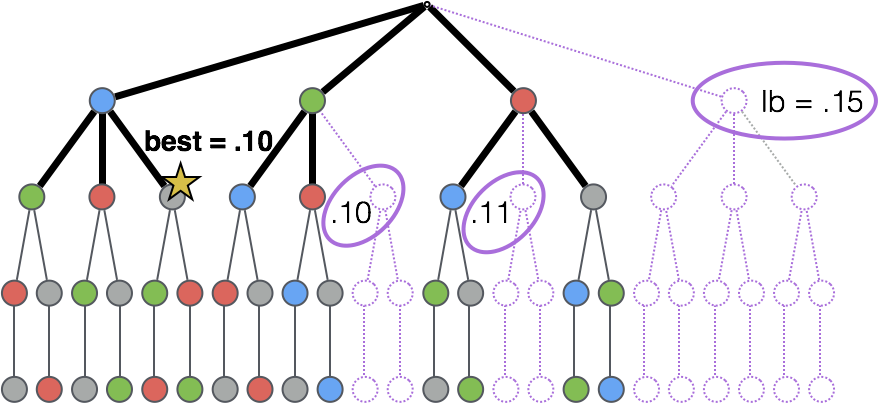
\includegraphics[width=0.5\textwidth]{figs/ela_branch-and-bound-tree-pruned.png}
\caption[Objective bound]{This tree shows the objective bound in action. Our best objective seen is the rule list (blue, gray) with an objective of $0.10$. Any rule lists with lower bound greater than this objective--(gray), (red, green), (green, gray) can be pruned and
\label{fig:objective-bound}}
\end{figure}

\subsubsection{Permutation Bound}

As defined above, every sample is captured by precisely one rule--any sample that is caught by rule A in the rule list AB cannot be caught by rule B. 
Now consider a permutation of the rule list AB: the rule list BA.
Any samples that are captured by either rule A or B but not both will be captured identically in both rule lists.
Samples that are captured by both rules will again be captured the same in both rule lists, though they may be predicted differently in the two rule lists.
Thus, regardless of the order in which the rules appear, rule lists AB and BA will capture exactly the same set data.
They will differ only in which rules capture which samples and therefore their accuracy may differ. 
We can use this knowledge to create a bound as follows.
If we know that the lower bound of AB is better than the lower bound of BA, we can eliminate from consideration all rule lists beginning with BA.
This is due to the fact that any corresponding rule list beginning with AB will capture exactly the same samples as the equivalent rule list beginning with BA but will have a better objective function.
We can eliminate all but one permutation of a given set of rules using this principle.

\subsubsection{Support Bound}
Due to our regularization term in calculating our objective function, adding a rule that does little to help our accuracy will actually be harmful to the overall objective score.
This allows us to place a bound intrinsic to the rule we're proposing adding.
We only consider adding rules that have capture enough data points correctly to overcome the regularization term.
Even though all rules have at least that support in the first case, as our rule lists get longer many rules do not capture enough points that haven't already been captured.

\subsubsection{Equivalent Points Bound}
This bound relies on the structure of our dataset.
In our dataset, we may encounter two data points that have the same features but different labels.
Thus, any rule that classifies one of the data points will also classify the other data point, but it is impossible to correctly predict both data points.
For a given class of equivalence points, therefore, we know that we will mispredict all of the points with a minority label.
We can thus update our lower bound to, by assuming that all uncaptured data will be correctly predicted only if it is not an equivalent point with a minority label.
This gives us much tighter lower bounds and in practice allows us to prune much more efficiently.

\subsection{Curiosity}
We have a number of different ways to explore the search space (see \ref{queue}).
Some of them, such as BFS prioritize exploration over exploitation.
Others, such as ordering by lower bound ensure that we are purely exploiting the best prefixes that we've seen.
We define a new metric, \textit{curiosity}, that is a function of both the lower bound and the number of samples captured.
This allows it to blend together both exploration and exploitation.

\subsection{Remaining Search Space}
Throughout this work, we will want to track how effective our bounds and other optimizations are.
One metric for tracking that will be seeing how quickly we reduce the remaining search space.
We start with a combinatorially large search space, but quickly prune it down.
The way we calculate the currently remaining search space is by looking at all of the leaves of the queue and seeing how much each leaf could potentially be expanded.
Due to our regularization term, we are able to bound the maximum length of a prefix as our best objective gets updated.